\newpage
\subsection*{Question 1}

\begin{enumerate}[label={(\alph*)}]
    \item We assume that we have an ISAM structure with 4 entries per page. While 25 is directly inserted in a page, 35 will be an overflow node. New ISAM structure is shown bellow. 
    
        \begin{center}
        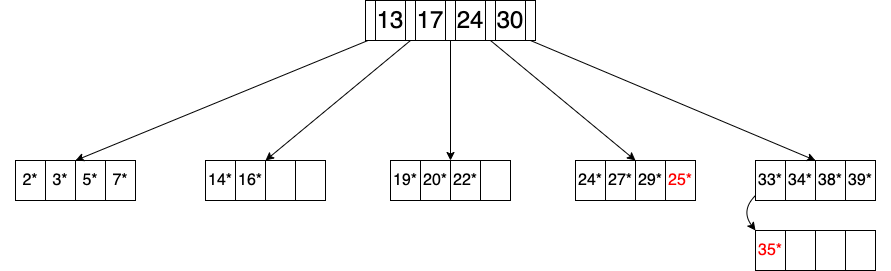
\includegraphics[width=1\textwidth]{img/img1.png}
        \end{center}
        
    \item The correct tree is Tree B
    
    \item The correct tree is Tree A
    
    \item Since a the borrowing should occur from the right sibling, none of the trees are correct. Bellow is shown the correct $B^+$-tree resulting from deleting of $16^*$ and then borrowing a node from the right sibling;
        \begin{center}
            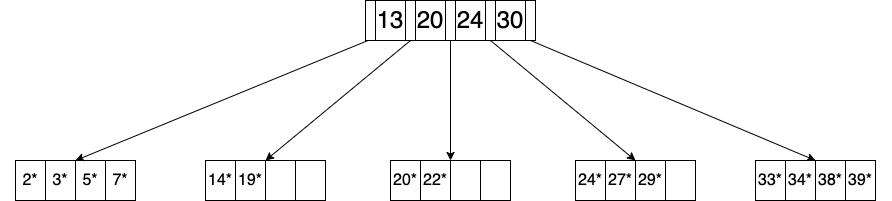
\includegraphics[width=1\textwidth]{img/img4.png}
        \end{center}
    
\end{enumerate}